\documentclass{beamer}
\usepackage{pgfpages}
%%\setbeameroption{show notes on second screen=left} %enable for notes
\usepackage{graphicx}
\usepackage{xcolor}
\usepackage{listings}
\usepackage{hyperref}
\lstset{language=python,frame=single}
\usepackage{verbatim}
\usepackage{apacite}
\usepackage{subcaption}
\usepackage{amsmath}
\usepackage{relsize}

\usetheme{Madrid}
%%\AtBeginSection[]
%%{
%%  \begin{frame}
%%    \frametitle{Table of Contents}
%%    \tableofcontents[currentsection]
%%  \end{frame}
%%}

%%\let\olditem\item
%%\renewcommand{\item}{\vspace{0.5\baselineskip}\olditem}
\begin{document}

\title{Learning Parallels}
\subtitle{Analogies emerge from learning dynamics in neural networks}
\author{Andrew Lampinen}
\date{3/7/2017}
\frame{\titlepage}


\section{Introduction}
\begin{frame}{Last time...}
\begin{center}
\includegraphics[width = 0.4\textwidth]{hexagon_arrow.png}
\end{center}
\end{frame}

\begin{frame}{Analogy, Transfer, and Cognition}
\begin{itemize}
    \item<1-> ``What makes humans smart is (1) our exceptional ability to learn by analogy'' \cite{Gentner2003} 
    \item<2-> ``Significant transfer is probably rare and accounts for very little human behavior. ... We generally do what we have learned to do and no more.'' \cite{Detterman1993}
    \item<3-> ``We found evidence for analogical transfer from a concrete, highly perceptual system to a very dissimilar domain and task ... participants transfer was independent of their explicit reports [of awareness of the analogy between the tasks].'' \cite{Day2011}
    \item<4-> ``Our proposal is to view transfer from the perspective of preparation for future learning (PFL).'' \cite{Bransford1999} 
\end{itemize}
\note{Fortunately, there's a great deal of agreement in the field}
\end{frame}

\begin{frame}{Analogy, Transfer, and Neural Networks}
If and when analogical reasoning is important for human cognition, how can we solve the combinatorially explosive analogical mapping problem? Perhaps using neural networks to do amortized inference. 
\begin{itemize}
    \item<2-> Zero-shot machine translation \cite{Johnson2016}
    \item<3-> Training machine translation on image captioning tasks improves performance \cite{Luong2016} 
    \item<4-> Hinton family tree task \cite{Hinton1986}
    \begin{center}
	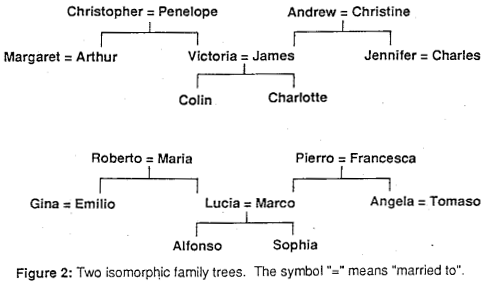
\includegraphics[width = 0.4\textwidth]{../writing/cogsci_2017/figures/hinton_family_tree_figure.png}
    \end{center}
\end{itemize}
\end{frame}

\section{Modeling: A toy task}
\begin{frame}{A toy task}
Learning which letters can follow other letters:\vspace{-2em}
\begin{center}
\[
\begin{array}{c|cccccc} 
& P & D & S & \pi & \delta & \sigma \\
\hline
R & 1 & 1 & 0 & 0 & 0 & 0 \\
L & 1 & 0 & 1 & 0 & 0 & 0 \\
\rho & 0 & 0 & 0 & 1 & 1 & 0\\
\lambda & 0 & 0 & 0 & 1 & 0 & 1\\
\end{array} 
\]
\end{center}
\only<2->{How, when, and why will a neural network exploit the analogy between the Latin and Greek letters?}
\end{frame}

\section{(A Little) Theory}
\begin{frame}{Linear Analyses?}
\begin{itemize}
    \item<1-> In a linear network, learning is driven entirely by features of the SVD (Singular Value Decomposition) of the Input/Output (I/O) mapping \cite{Saxe2013}.
    \item<2-> Can we analyze learning of analogous structure in a linear framework?
    \item<3-> \textbf{NO,} in the SVD of a block-diagonal matrix, the modes occur within the blocks, thus \textbf{a linear network cannot represent shared structure at convergence.}
\only<4->{
\begin{figure}
\centering
\begin{subfigure}{0.2\textwidth}
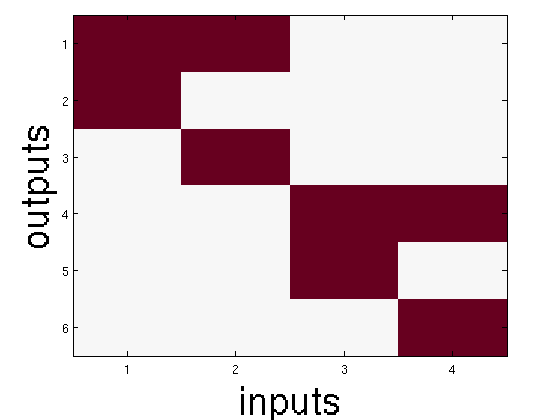
\includegraphics[width=\textwidth]{../writing/cogsci_2017/figures/nonlinear_IO.png}
\caption{$\Sigma_{IO}$}
\end{subfigure}
\raisebox{0.5em}{\!\!\huge{$=$}\!\!}
\begin{subfigure}{0.2\textwidth}
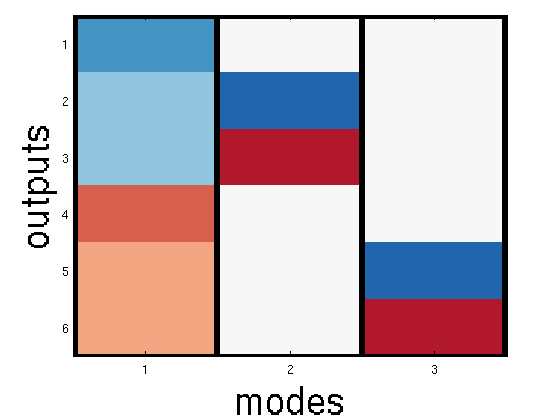
\includegraphics[width=\textwidth]{../writing/cogsci_2017/figures/U_nl.png}
\caption{$U$}
\end{subfigure}
\raisebox{0.5em}{\!\!\LARGE{$\times$}\!\!}
\begin{subfigure}{0.2\textwidth}
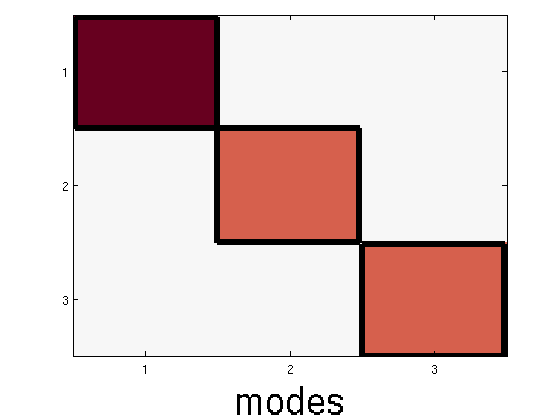
\includegraphics[width=\textwidth]{../writing/cogsci_2017/figures/S_nl.png}
\caption{$S$}
\end{subfigure}
\raisebox{0.5em}{\!\!\LARGE{$\times$}\!\!}
\begin{subfigure}{0.2\textwidth}
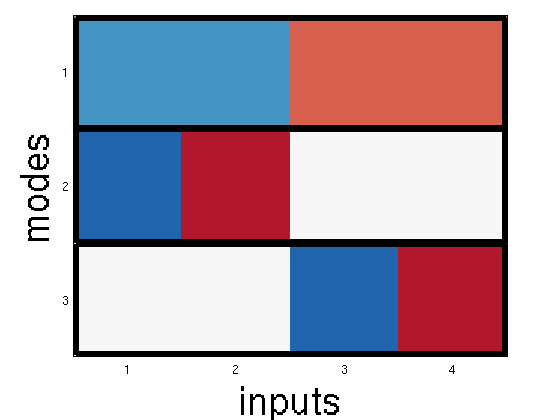
\includegraphics[width=\textwidth]{../writing/cogsci_2017/figures/V_nl.png}
\caption{$V^T$}
\end{subfigure}
\end{figure}
}
\item<5-> This also means that a linear network \textbf{cannot achieve as parsimonious a solution as a nonlinear network}, because it must solve each copy of a problem separately rather exploiting analogies between them.
\end{itemize}
\end{frame}


\begin{frame}{Linearized analysis}
\begin{columns}
    \column{0.5\textwidth}
	However, we would still like to use linear analysis tools, so:
	\begin{itemize}
	    \item<2-> Linearized analysis: SVD of linear portion of network. 
	\end{itemize}
    \column{0.5\textwidth}
	\begin{center}
	    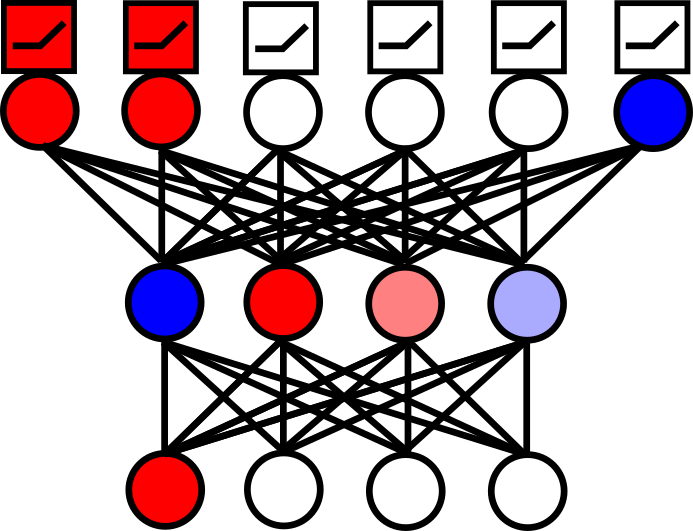
\includegraphics[width=0.8\textwidth]{../writing/cogsci_2017/figures/network_diagram.png}
	\end{center}
\end{columns}
\end{frame}

\section{The Return of the Toy Task}
\begin{frame}{Toy task}
What solutions does the network discover?
\begin{columns}
    \column{0.5\textwidth}
	    \[
	    \begin{array}{c|cccccc} 
	    & P & D & S & \pi & \delta & \sigma \\
	    \hline
	    R & 1 & 1 & 0 & 0 & 0 & 0 \\
	    L & 1 & 0 & 1 & 0 & 0 & 0 \\
	    \rho & 0 & 0 & 0 & 1 & 1 & 0\\
	    \lambda & 0 & 0 & 0 & 1 & 0 & 1\\
	    \end{array} 
	    \]
    \column{0.5\textwidth}
	\begin{center}
	    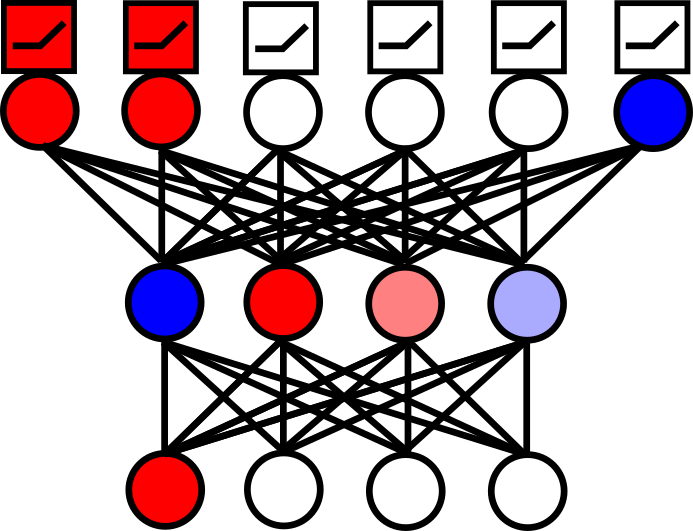
\includegraphics[width=0.8\textwidth]{../writing/cogsci_2017/figures/network_diagram.png}
	\end{center}
\end{columns}
\note{note that no weights are shared between the two tasks!}
\end{frame}

\begin{frame}{Toy task solutions}
Most commonly with ReLU, the network learns an offset structure, resulting in the following linearized I/O mapping (or a symmetric analog): 
\[
\left[ \begin{matrix} 
1 & 1 & 0 & 0 & 0 & -1 \\
1 & 0 & 1 & 0 & -1 & 0 \\
 0 & 0 & -1 & 1 & 1 & 0\\
 0 & -1 & 0 & 1 & 0 & 1\\
\end{matrix}  \right] 
\]
\only<2->{(This is certainly not the only solution that can occur, but this happens about 75\% of the time. The remaining 25\% no analogy is discovered.)}
\end{frame}

\begin{frame}{Comparing SVDs}
\begin{itemize}
    \item<1-> Non-linear I/O Mapping
    \only<1->{
    \begin{figure}
    \centering
    \begin{subfigure}{0.2\textwidth}
    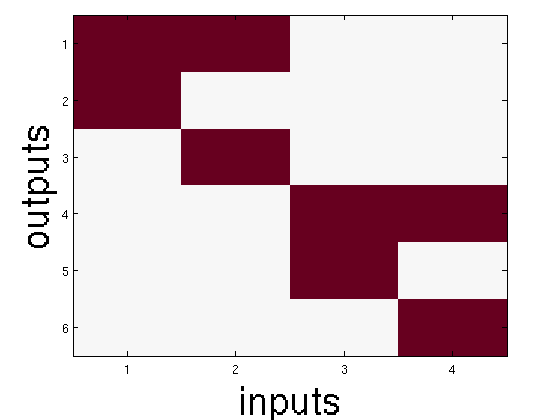
\includegraphics[width=\textwidth]{../writing/cogsci_2017/figures/nonlinear_IO.png}
    \caption{$\Sigma_{IO}$}
    \end{subfigure}
    \raisebox{0.5em}{\!\!\huge{$=$}\!\!}
    \begin{subfigure}{0.2\textwidth}
    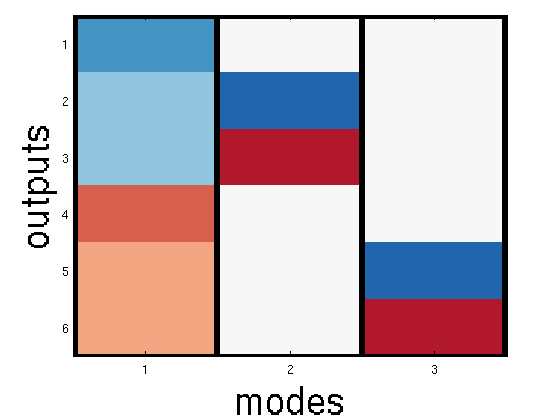
\includegraphics[width=\textwidth]{../writing/cogsci_2017/figures/U_nl.png}
    \caption{$U$}
    \end{subfigure}
    \raisebox{0.5em}{\!\!\LARGE{$\times$}\!\!}
    \begin{subfigure}{0.2\textwidth}
    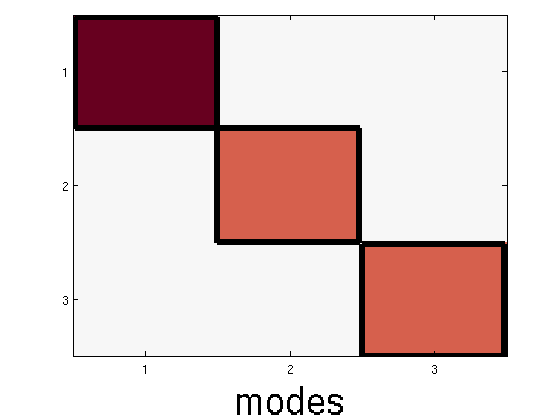
\includegraphics[width=\textwidth]{../writing/cogsci_2017/figures/S_nl.png}
    \caption{$S$}
    \end{subfigure}
    \raisebox{0.5em}{\!\!\LARGE{$\times$}\!\!}
    \begin{subfigure}{0.2\textwidth}
    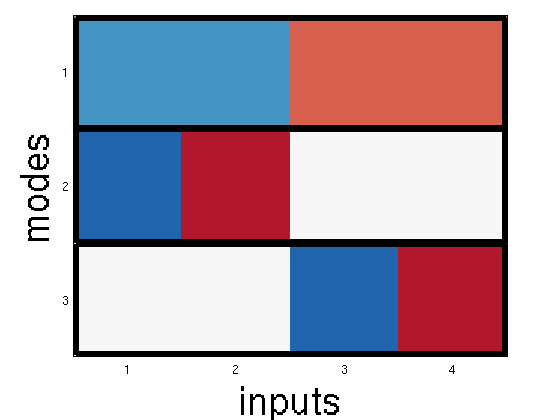
\includegraphics[width=\textwidth]{../writing/cogsci_2017/figures/V_nl.png}
    \caption{$V^T$}
    \end{subfigure}
    \end{figure}
    }
    \item<2-> Linearized I/O Mapping
    \only<2->{
    \begin{figure}
    \centering
    \begin{subfigure}{0.2\textwidth}
    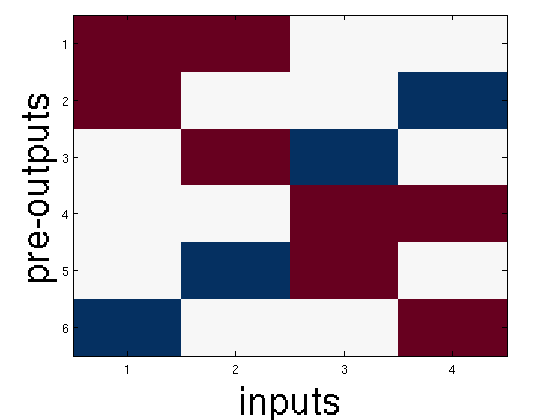
\includegraphics[width=\textwidth]{../writing/cogsci_2017/figures/linearized_IO.png}
    \caption{$\Sigma_{IO}$}
    \end{subfigure}
    \raisebox{0.5em}{\!\!\huge{$=$}\!\!}
    \begin{subfigure}{0.2\textwidth}
    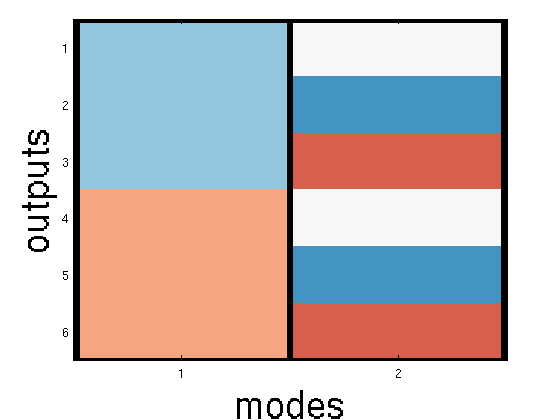
\includegraphics[width=\textwidth]{../writing/cogsci_2017/figures/U_lz.png}
    \caption{$U$}
    \end{subfigure}
    \raisebox{0.5em}{\!\!\LARGE{$\times$}\!\!}
    \begin{subfigure}{0.2\textwidth}
    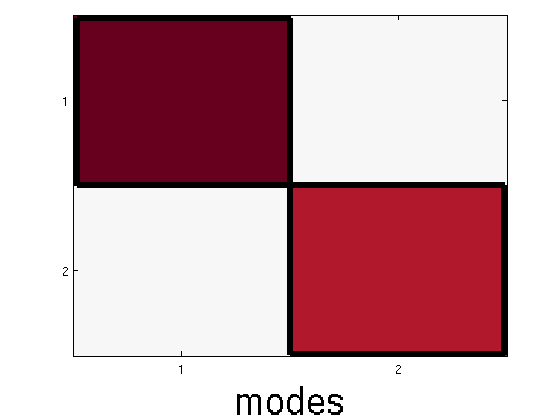
\includegraphics[width=\textwidth]{../writing/cogsci_2017/figures/S_lz.png}
    \caption{$S$}
    \end{subfigure}
    \raisebox{0.5em}{\!\!\LARGE{$\times$}\!\!}
    \begin{subfigure}{0.2\textwidth}
    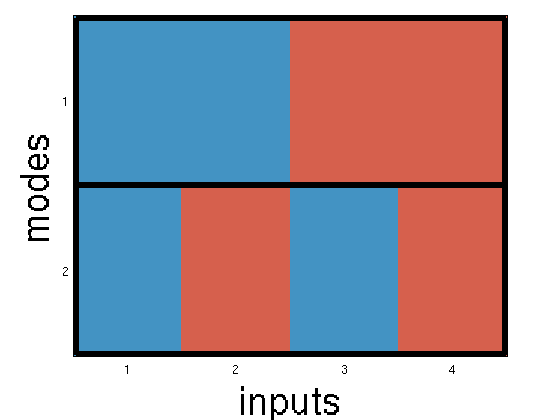
\includegraphics[width=\textwidth]{../writing/cogsci_2017/figures/V_lz.png}
    \caption{$V^T$}
    \end{subfigure}
    \end{figure}
    }
    \item<3-> Linearized I/O shows network has captured the shared structure!
\end{itemize}
\note{Can interpret the top SVD in several ways, as the task that a linear network solves, or as the task that a non-linear netwokr begins solving when it is still in the linear regime. Note more parsimonious solutions available with linearized mapping.}
\end{frame}

\begin{frame}{Learning dynamics}
But why and how does this occur? The linearized SVD cannot tell us, but the progression is fairly consistent: \\[11pt]
\begin{columns}
    \column{0.45\textwidth}
    \uncover<2->{Initial:{\relsize{-1}
    \[ 
    \left[ \begin{matrix} 
    0 & 0 & 0 & 0 & 0 & 0 \\
    \vdots & \vdots &\vdots &\vdots &\vdots &\vdots \\
     0 & 0 & 0 & 0 & 0 & 0\\
    \end{matrix}  \right] 
    \] 
    }}
    \uncover<4->{Base rates by domain:{\relsize{-1}
    \[
    \left[ \begin{matrix} 
    1 & 0.5 & 0.5 & 0 & 0 & 0 \\
    1 & 0.5 & 0.5 & 0 & 0 & 0 \\
    0 & 0 & 0 & 1 & 0.5 & 0.5  \\
    0 & 0 & 0 & 1 & 0.5 & 0.5  \\
    \end{matrix}  \right] 
    \]
    }
    }
    \column{0.45\textwidth}
    \uncover<3->{Base rates:{\relsize{-1}
    \[ 
    \left[ \begin{matrix} 
    0.5 & 0.25 & 0.25 & 0.5 & 0.25 & 0.25 \\
    \vdots & \vdots &\vdots &\vdots &\vdots &\vdots \\
     0.5 & 0.25 & 0.25 & 0.5 & 0.25 & 0.25\\
    \end{matrix}  \right] 
    \] 
    }}
    \uncover<5->{Solution with offsets:{\relsize{-1}
    \[
    \left[ \begin{matrix} 
    1 & 1 & 0 & 0 & 0 & -1 \\
    1 & 0 & 1 & 0 & -1 & 0 \\
     0 & 0 & -1 & 1 & 1 & 0\\
     0 & -1 & 0 & 1 & 0 & 1\\
    \end{matrix}  \right] 
    \]
    }}
\end{columns}
\uncover<6->{For all but the last step, linear network learning dynamics are very similar! Do they also start to extract some shared structure?}
\end{frame}

\begin{frame}{Learning dynamics}
In fact, linear networks begin to extract the shared structure as well, but must discard it to achieve their optimal solution.
\begin{center}
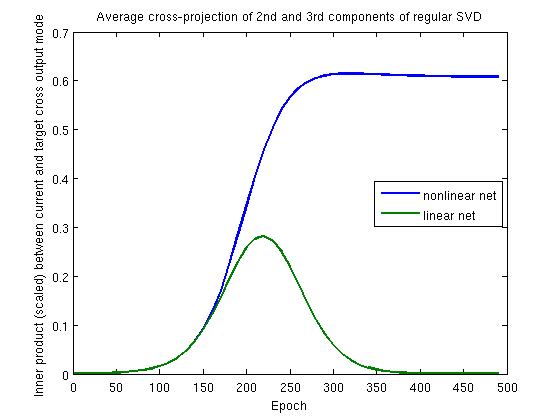
\includegraphics[width=0.7\textwidth]{../writing/cogsci_2017/figures/SVD_cross_projection_learning.png}
\end{center}
\note{What the fuck is up with this plot? What does it actually mean?}
\end{frame}

\begin{frame}{Learning dynamics}
Why? \\[5pt]
\begin{columns}
    \column{0.45\textwidth}
    \only<1->{Base rates by domain:{\relsize{-1}
    \[
    \left[ \begin{matrix} 
    1 & 0.5 & 0.5 & 0 & 0 & 0 \\
    1 & 0.5 & 0.5 & 0 & 0 & 0 \\
    0 & 0 & 0 & 1 & 0.5 & 0.5  \\
    0 & 0 & 0 & 1 & 0.5 & 0.5  \\
    \end{matrix}  \right] 
    \]
    }
    }
    \column{0.45\textwidth}
    \only<2->{Base rates + a little shared structure{ \relsize{-1}
    \[
    \left[ \begin{matrix} 
    1 & 0.6 & 0.4 & 0 & 0.1 & -0.1 \\
    1 & 0.4 & 0.6 & 0 & -0.1 & 0.1 \\
    0 & 0.1 & -0.1 & 1 & 0.6 & 0.4  \\
    0 & -0.1 & 0.1 & 1 & 0.4 & 0.6  \\
    \end{matrix}  \right] 
    \] 
    }}
\end{columns}
\uncover<3->{ More explicitly, this emerges naturally from SGD (weight updates for a unit on an example are proportional to the product of the output error and the unit's activation)  
{ \relsize{-1}
\[
\begin{array}{cccccc||c||cccccc} 
\multicolumn{6}{c||}{\text{output error}}  & \text{unit}  & \multicolumn{6}{c}{\text{unit output weight updates}} \\
\hline
 0 & + & - & 0 & 0 & 0  &   +    &  0 & + & - & 0 & 0 & 0   \\
0 & - & + & 0 & 0 & 0  &   -  & 0 & + & - & 0 & 0 & 0   \\
 0 & 0 & 0 & 0 & + & - &   +   &  0 & 0 & 0 & 0 & + & - \\
 0 & 0 & 0 & 0 & - & +  &  - &  0 & 0 & 0 & 0 & + & - \\
\hline
\multicolumn{7}{r}{\text{net output weight update:}} &   0 & + & - & 0 & + & - \\
\end{array} 
\]
}
} 
\note{So network will exploit the analogy to reduce error, even though no weights are shared, and even if it must discard it in the linear case.}
\end{frame}

\section{A more interesting example: Hinton's family tree task}
\begin{frame}{Hinton family tree task}
\begin{columns}
    \column{0.5\textwidth}
    \begin{center}
	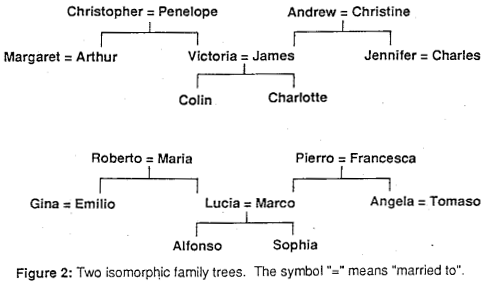
\includegraphics[width = \textwidth]{../writing/cogsci_2017/figures/hinton_family_tree_figure.png}
    \end{center}
    \column{0.5\textwidth}
    \begin{center}
	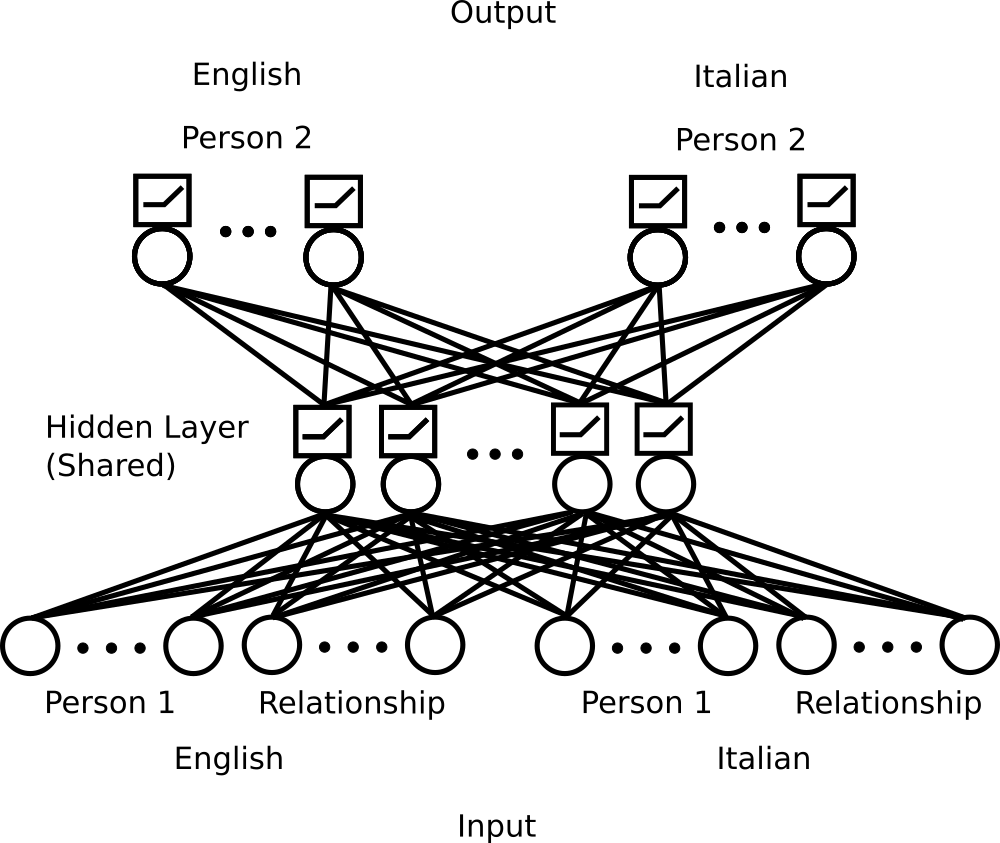
\includegraphics[width = \textwidth]{../writing/cogsci_2017/figures/family_tree_network_diagram.png}
    \end{center}
\end{columns}
\begin{itemize}
\item<2-> Our network is simplified from Hinton's, and tasks are completely separated.
\end{itemize}
\end{frame}

\begin{frame}{Hinton family tree task: Problems}
A few problems:
\begin{itemize}
    \item<2-> Task is not linearly separable, so we have multiple non-linearities, so how to perform analysis?
    \begin{itemize}
	\item<3-> The simple approach we took is just to perform the linearized analysis at each layer. 
    \end{itemize}
    \item<4-> Multiple analogies exist between family trees (for example flip left to right and reverse genders) 
    \begin{itemize}
	\item<5-> Include both these analogies in our analysis. 
    \end{itemize}
    \item<6-> Cannot simply ``eyeball'' structure extraction here, need a principled measure of shared structure extraction. 
    \begin{itemize}
	\item<7-> Use a permutation test on each SVD mode to see whether the domains share more structure in this mode than would be expected by chance. 
    \end{itemize}
\end{itemize}
\only<4> {
\vspace{-80pt}
\begin{center}
    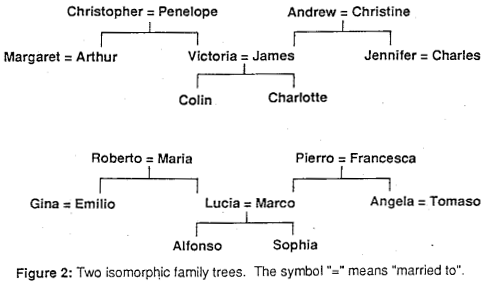
\includegraphics[width = 0.4\textwidth]{../writing/cogsci_2017/figures/hinton_family_tree_figure.png}
\end{center}
}
\note{Hinton shared relationship inputs, and had shared hidden layers, but we want to strip down to see if the analogies will emerge from the learning dynamics like in the above task.}
\end{frame}

\begin{frame}{Results}
Significant amounts of shared structure extraction!\\[11pt]
\begin{columns}
\column{0.45\textwidth}
    \uncover<2->{
    First layer input modes:
    \begin{center}
    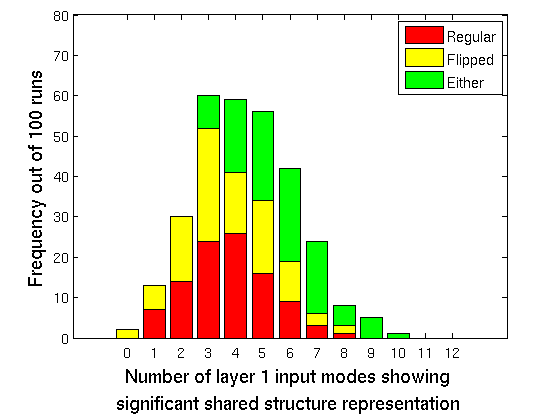
\includegraphics[width=1.1\textwidth]{../writing/cogsci_2017/figures/ft_input_mode_significance_hist.png} 
    \end{center}
    }

\column{0.45\textwidth}
    \uncover<3->{
    Second layer output modes:
    \begin{center}
    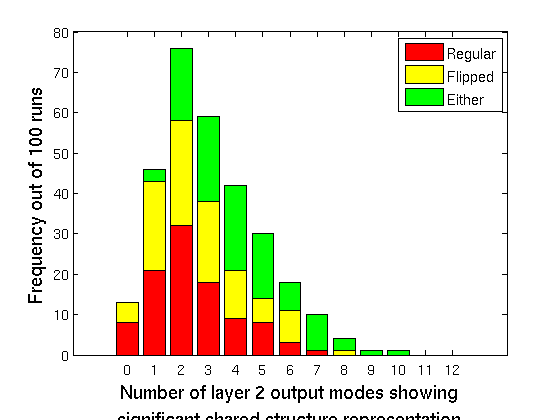
\includegraphics[width=1.1\textwidth]{../writing/cogsci_2017/figures/ft_output_mode_significance_hist.png} 
    \end{center}
    }
\end{columns}
\end{frame}

\begin{frame}{Shared structure highlights:}
The input layers had:
\begin{itemize}
    \item<1-> A median of 6 modes showing significant extraction of the analogy to either the regular or flipped mapping (null: only 0.01\% of runs with 6 significant modes, median 0).
    \item<2-> 3 or more significant components from at one of the mappings alone in 95\% of the runs (null: in 4\% of runs).
    \item<3-> 3 or more significant components overall in all of the runs (null: in 3\% of runs).
\end{itemize}
\uncover<4->{Shared structure extraction appears \textbf{more consistent in a more complex task} than it was in the toy task}
\end{frame}
\section{Conclusions}

\begin{frame}{Results summary}
\begin{itemize}
    \item<1-> We outlined a new analysis method for non-linear neural networks. 
    \item<2-> Used this in a toy task to show that analogies between non-overlapping tasks emerge naturally from learning dynamics. 
    \item<3-> Used in a more complicated task, and found that extraction of the analogies was even more consistent than on the toy task. 
    \item<4-> This extraction of analogies does not even require shared weights, learning (or replaying) the tasks together suffices.
    \item<5-> This provides a good model for ``slow'' human analogical reasoning and transfer, including:
    \begin{itemize}
	\item<6-> Benefits of multiple mutually supporting tasks.
	\item<7-> Preparation for future learning.
	\item<8-> Possible amortized inference about analogies.
    \end{itemize}
\end{itemize}
\end{frame}

\section{Thank you}
\begin{frame}{Acknowledgements}
Thanks to:
\begin{itemize}
    \item Co-authors: Shaw Hsu \& Jay McClelland
    \item The rest of the lab for helpful conversations and feedback. 
\end{itemize}
\end{frame}

\section{References}
\begin{frame}[allowframebreaks]
\frametitle{References}
\bibliographystyle{apacite}
\bibliography{shared_reps}
\end{frame}
\end{document}
